\documentclass{article}
\usepackage{graphicx} 
\usepackage{amsfonts} 
\usepackage{amsmath}
\usepackage{multirow}
\usepackage{tikz}
\usepackage{polski}
\usepackage{mathtools}
\usepackage{hyperref}
\usepackage{breqn}

\title{ Oczekiwana liczba podgrafów Kuratowskiego \newline w grafie losowym Barabasi Albert $G^n_m$ }

\author{}

\date{}

\begin{document}

\maketitle

\section{Oznaczenia}
\begin{itemize}
  \item $G_{m}^{n}$ - graf Barabasi Albert o końcowej liczbie wierzchołków $n$ oraz $m$ dodawanych krawędziach do każdego wierzchołka
  \item $V^{+}(G)$ - wierzchołki z których krawędzie wychodzą
  \item $V^{-}(G)$ - wierzchołki do których krawędzie prowadzą
  \item $d_{G}^{in}(v)$ - stopień wejściowy
  \item $d_{G}^{out}(v)$ - stopień wyjściowy
  \item $d_{G}(v) = d_{G}^{in}(v) + d_{G}^{out}(v)$
  \item $C_{G}(t)$ - liczba 'przecięć' $t$, tj. liczba krawędzi $(u,v)$ takich że $u \leq t \leq v$
\end{itemize}

Uwaga: Pętle dodają jeden do $d_{G}^{in}(v)$ oraz jeden do $d_{G}^{out}(v)$ <br>

\section{Metoda}
Na podstawie \href{https://www.stat.berkeley.edu/users/aldous/Networks/boll1.pdf}
{\textit{Mathematical results on scale-free random graphs}} (paragraf 15 i 12)
mamy wzory wyrażające prawdopodobieństwo $p_H$ występowanie pewnego podgrafu $H$ w grafie $G^n_1$ 
opisanego jako zbiór krawędzi łączących konkretne wierzchołki:
% \begin{dmath}
%   p_H = \prod_{v \in V^{-}(H)} d_{H}^{in}(v)! \prod_{v \in V^{+}(H)} \frac{1}{2v - 1} \prod_{v \notin V^{+}(H)} (1 + \frac{C_{H}(v)}{2v-1})
% \end{dmath}

\begin{dmath}
  p_H = \prod_{v \in V^{-}(H)} d_{H}^{in}(v)! \prod_{ij \in E(H)} \frac{1}{2 \sqrt{ij}} \exp(O(\sum_{i \in V(H)}\frac{C_H(i)^2}{i}))
\end{dmath}
Aby opisać graf $G^n_m$ za pomocą modelu z parametrem $m=1$ budujemy graf $G^{m \cdot n}_1$
taki że każde kolejne $m$ wierzchołków utożsamiamy jako jeden wierzchołek reprezentujący ten z grafu z dowolną wartością $m$.
\newline
Wymaganiami podanych wyżej wzorów jest to aby każda krawędź była zorientowana od wierzchołka o większym numerze to do tego z mniejszym
oraz liczba krawędzi wychodzących nie była większa niż 1 - wówczas osadzenie takiego podgrafu w grafie losowym jest możliwe.

\section{Oczekiwana liczba $K_5$}
Niech $a$,$b$,$c$,$d$,$e$ będą wierzchołkami w $G_m^n$ tworzącymi potencjalne $K_5$. 
Bierzemy graf $G = G_1^{n \cdot m}$ oraz graf  $H = K_5$. Nadajemy oznaczenia. Wówczas:
\begin{itemize}
  \item $V(G) = \{1, 2, \ldots n \cdot m\}$
  \item $E(H) = \{(o_{x_1}, i_{y_1}), (o_{x_2}, j_{y_2}), (o_{x_3}, k_{y_3}), (o_{x_4}, l_{y_4}), (l_{x_5}, i_{y_5}), (l_{x_6}, j_{y_6}),  \newline (l_{x_7}, k_{y_7}), (k_{x_8}, i_{y_8}), (k_{x_9}, j_{y_9}), (j_{x_{10}}, i_{y_{10}})\}$
    \subitem $a < b < c < d < e$
    \subitem $m \cdot (a-1) \leq i_1,i_2,i_3,i_4 \leq m \cdot a$
    \subitem $m \cdot (b-1) \leq j_1,j_2,j_3,j_4 \leq m \cdot b$
    \subitem $m \cdot (c-1) \leq k_1,k_2,k_3,k_4 \leq m \cdot c$
    \subitem $m \cdot (d-1) \leq l_1,l_2,l_3,l_4 \leq m \cdot d$
    \subitem $m \cdot (e-1) \leq o_1,o_2,o_3,o_4 \leq m \cdot e$
\end{itemize}

\begin{dmath}
  \mathbb{E}[K_5] = \sum_{K_5^* \in \mathbb{K}_5} \mathbb{E}[K_5^*] =
  \sum_{K_5^* \in \mathbb{K}_5} \sum_{1 \leq a < b < c < d < e \leq n} \#K_{a,b,c,d,e}^* \cdot p_{K_{a,b,c,d,e}^*}
\end{dmath}
gdzie $K_5^*$ to konkretna instancja $K_5$ z ustalonymi stopniami wyjściowymi \newline
a $K_{a,b,c,d,e}^*$ to $K_5^*$ z ustalonymi indeksami wierzchołków na $a,b,c,d,e$.

\subsection{Przykładowe $K_{a,b,c,d,e}$ dla $m=4$}
\begin{figure}[h]
  \centering
  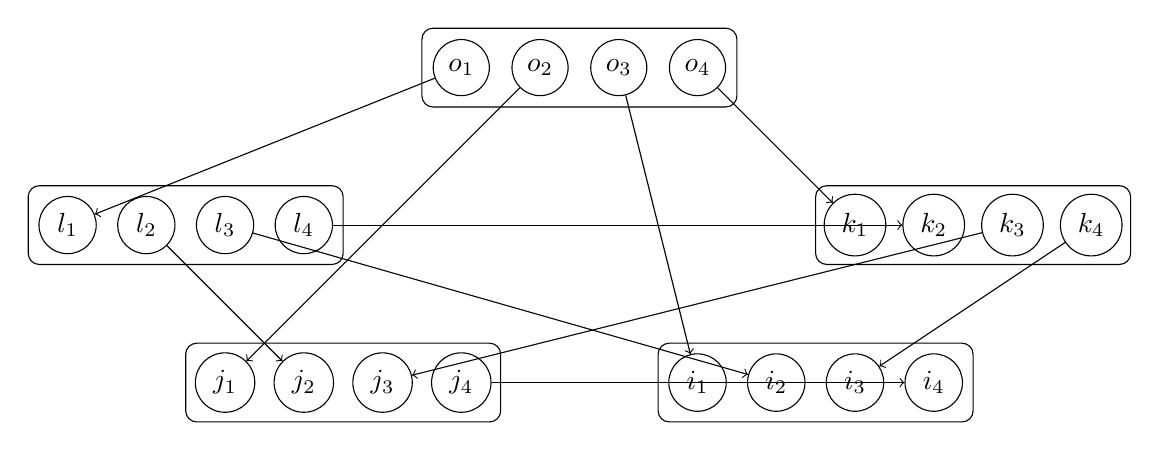
\begin{tikzpicture}
    \draw[rounded corners] (0, 0) rectangle (4, 1) {};
    \node[draw=black, shape=circle, minimum size=0.5cm] (o1) at (0.5,0.5) {$o_1$};
    \node[draw=black, shape=circle, minimum size=0.5cm] (o2) at (1.5,0.5) {$o_2$};
    \node[draw=black, shape=circle, minimum size=0.5cm] (o3) at (2.5,0.5) {$o_3$};
    \node[draw=black, shape=circle, minimum size=0.5cm] (o4) at (3.5,0.5) {$o_4$};

    \draw[rounded corners] (-5, -2) rectangle (-1, -1) {};
    \node[draw=black, shape=circle, minimum size=0.5cm] (l1) at (-4.5, -1.5) {$l_1$};
    \node[draw=black, shape=circle, minimum size=0.5cm] (l2) at (-3.5, -1.5) {$l_2$};
    \node[draw=black, shape=circle, minimum size=0.5cm] (l3) at (-2.5, -1.5) {$l_3$};
    \node[draw=black, shape=circle, minimum size=0.5cm] (l4) at (-1.5, -1.5) {$l_4$};

    \draw[rounded corners] (5, -2) rectangle (9, -1) {};
    \node[draw=black, shape=circle, minimum size=0.5cm] (k1) at (5.5, -1.5) {$k_1$};
    \node[draw=black, shape=circle, minimum size=0.5cm] (k2) at (6.5, -1.5) {$k_2$};
    \node[draw=black, shape=circle, minimum size=0.5cm] (k3) at (7.5, -1.5) {$k_3$};
    \node[draw=black, shape=circle, minimum size=0.5cm] (k4) at (8.5, -1.5) {$k_4$};

    \draw[rounded corners] (-3, -4) rectangle (1, -3) {};
    \node[draw=black, shape=circle, minimum size=0.5cm] (j1) at (-2.5, -3.5) {$j_1$};
    \node[draw=black, shape=circle, minimum size=0.5cm] (j2) at (-1.5, -3.5) {$j_2$};
    \node[draw=black, shape=circle, minimum size=0.5cm] (j3) at (-0.5, -3.5) {$j_3$};
    \node[draw=black, shape=circle, minimum size=0.5cm] (j4) at (0.5, -3.5) {$j_4$};

    \draw[rounded corners] (3, -4) rectangle (7, -3) {};
    \node[draw=black, shape=circle, minimum size=0.5cm] (i1) at (3.5, -3.5) {$i_1$};
    \node[draw=black, shape=circle, minimum size=0.5cm] (i2) at (4.5, -3.5) {$i_2$};
    \node[draw=black, shape=circle, minimum size=0.5cm] (i3) at (5.5, -3.5) {$i_3$};
    \node[draw=black, shape=circle, minimum size=0.5cm] (i4) at (6.5, -3.5) {$i_4$};

    \draw [->] (o1) -- (l1);
    \draw [->] (o2) -- (j1);
    \draw [->] (o3) -- (i1);
    \draw [->] (o4) -- (k1);
    \draw [->] (l2) -- (j2);
    \draw [->] (l3) -- (i2);
    \draw [->] (l4) -- (k2);
    \draw [->] (k3) -- (j3);
    \draw [->] (k4) -- (i3);
    \draw [->] (j4) -- (i4);

  \end{tikzpicture}
\end{figure}

\newpage

\subsection{Wyznaczanie liczby $K_{a,b,c,d,e}$}
Zakładamy że $m \geq 4$, ponieważ stopień wyjściowy nie może być większy niż 1 a maksymalna liczba wyjściowych krawędzi ze 'zgrupowanego' wierzchołka to 4.
\newline \newline
Początki krawędzi wychodzących wierzchołkom $o_x$ możemy przyporządkować na $m (m-1) (m-2) (m-3)$ sposoby.
Żadne krawędzie nie prowadzą do wierzchołków $o_x$.
\newline
Początki krawędzi wychodzących wierzchołkom $l_x$ możemy przyporządkować na $m (m-1) (m-2)$ sposobów.
Do $l_x$ prowadzi jedna krawędź, której koniec można wybrać na $m$ sposobów. Wówczas jeden wierzchołek ma stopień 1. 
\newline
Początki krawędzi wychodzących wierzchołkom $k_x$ możemy przyporządkować na $m (m-1)$ sposobów.
Do $k_x$ prowadzą dwie krawędzie, których końce można wybrać na:
\begin{itemize}
  \item $m (m-1)$ sposobów, wówczas dwa wierzchołki mają stopień 1.
  \item $m$ sposobów, wówczas jeden wierzchołek ma stopień 2.
\end{itemize}
Początki krawędzi wychodzących wierzchołkom $j_x$ możemy przyporządkować na $m$ sposobów.
Do $j_x$ prowadzą 3 krawędzie, których końce można wybrać na:
\begin{itemize}
  \item $m (m-1) (m-2)$ sposobów, wówczas 3 wierzchołki mają stopień 1.
  \item $3 \cdot m (m-1)$ sposobów, wówczas 1 wierzchołek ma stopień 2 i 1 ma stopień 1.
  \item $m$ sposobów, wówczas jeden wierzchołek ma stopień wyjściowy 3.
\end{itemize}
Żadne krawędzie nie wychodzą z $i_x$.
Do $i_x$ prowadzą 4 krawędzie, których końce można wybrać na:
\begin{itemize}
  \item $m (m-1) (m-2) (m-3)$ sposobów, wówczas 4 wierzchołki mają stopień 1.
  \item $\frac{1}{2} \cdot m (m-1) (m-2) \cdot \binom{4}{2} \cdot 2$ sposobów, wówczas 2 wierzchołki mają stopień 2 a 2 pozostałe stopień 1.
  \item $\frac{1}{2} \cdot m (m-1) \cdot \binom{4}{2}$ sposobów, wówczas 1 i 2 wierzchołek ma stopień 2.
  \item $4 \cdot m (m-1)$ sposobów, wówczas 1 wierzchołek ma stopień wyjściowy 3 i 1 ma stopień 1.
  \item $m$ sposobów, wówczas jeden wierzchołek ma stopień 4.
\end{itemize}
Mamy zatem $1 \cdot 2 \cdot 3 \cdot 5 = 30$ różnych konfiguracji wyborów końców krawędzi.

\newpage

\subsection{Wyznaczanie prawdopodobieństwa $p_{K_{a,b,c,d,e}}$}
Ponieważ liczba krawędzi $H$ jest stała to liczba $C_H$ jest ograniczona z góry przez stałą.
Gdy $n$ jest wystarczająco duże to ilorazy $\frac{C_H(i)^2}{i}$ będą bliskie zeru zatem ostatni z 3 czynników iloczynu można zaniedbać:
\begin{dmath}
  p_{K_{a,b,c,d,e}^*} = (\prod_{v \in V^{-}(H)} d_{H}^{in}(v)!) \frac{1}{2^{10}} \frac{1}{\sqrt{m^{20} a^4 b^4 c^4 d^4 e^4}} 
  = (\prod_{v \in V^{-}(H)} d_{H}^{in}(v)!) \frac{1}{2^{10}} \frac{1}{m^{10} a^2 b^2 c^2 d^2 e^2}
\end{dmath} 

\subsection{Wyznaczanie oczekiwanej liczby $K_5$}

\begin{dmath}
  \mathbb{E}[K_5] = \sum_{K_5^* \in \mathbb{K}_5} \sum_{1 \leq a < b < c < d < e \leq n} \#K_{a,b,c,d,e}^* \cdot p_{K_{a,b,c,d,e}^*}
  = \sum_{K_5^* \in \mathbb{K}_5} (\prod_{v \in V^{-}(H)} d_{H}^{in}(v)!) \cdot \frac{1}{2^{10} m^{10}} \cdot \#K_{a,b,c,d,e}^* \sum_{1 \leq a < b < c < d < e \leq n} \frac{1}{a^2 b^2 c^2 d^2 e^2}
  = \sum_{K_5^* \in \mathbb{K}_5} [(\prod_{v \in V^{-}(H)} d_{H}^{in}(v)!) \cdot \frac{1}{2^{10} m^{10}} \cdot \#K_{a,b,c,d,e}^*] \cdot (\frac{1}{5!})^2 \cdot (H^2_n)^5
\end{dmath}
gdzie $H^2_n$ to n-ta liczba harmoniczna drugiego rodzaju.
\newline \newline
Ostatecznie oczekiwana liczba $K_5$ w grafie $G_m^n$ wynosi:
\begin{dmath}
  \mathbb{E}[K_5] = \frac{(m^2-9)(m^2-4)^2(m^2-1)^3}{14745600 m^2} (H^2_n)^5
\end{dmath}

\newpage

\subsection{Eksperyment}
Dla stałej $\eta \approx \frac{1}{6.7}$ tak prezentuje się porównanie teorii $\eta \cdot \mathbb{E}[K_5]$ i eksperymentu:

\begin{figure}[h!]
  \centering
  \includegraphics[width=13cm]{../k5.png}
  \caption{Porównanie teorii i eksperymentu dla $K_{5}$ - 100 prób}
\end{figure}

\newpage

\section{Oczekiwana liczba $K_{3,3}$}
Niech $a,b,c,d,e,f$ będą wierzchołkami w $G_m^n$ tworzącymi potencjalne $K_{3,3}$. Bierzemy graf $G=G^{n \cdot m}_1$ oraz graf $H = K_{3,3}$. Wówczas:
\begin{itemize}
  \item $V(G) = \{ 1,2,\ldots n \cdot m \}$
  \item Jest 10 różnych ustawień krawędzi w zależności od tego podziału wierzchołków na 2 podzbiory:
    \subitem $E(H_1) = \{ (p_{x_1}, k_{y_1}), (p_{x_2}, j_{y_2}), (p_{x_3}, i_{y_3}), \newline (o_{x_4}, k_{y_4}), (o_{x_5}, j_{y_5}), (o_{x_6}, i_{y_6}), (l_{x_7}, k_{y_7}), (l_{x_8}, j_{y_8}), (l_{x_9}, i_{y_9}) \}$
    \subitem $E(H_2) = \{ (p_{x_1}, l_{y_1}), (p_{x_2}, j_{y_2}), (p_{x_3}, i_{y_3}), \newline (o_{x_4}, l_{y_4}), (o_{x_5}, j_{y_5}), (o_{x_6}, i_{y_6}), (k_{x_7}, l_{y_7}), (k_{x_8}, j_{y_8}), (k_{x_9}, i_{y_9}) \}$
    \subitem $E(H_3) = \{ (p_{x_1}, o_{y_1}), (p_{x_2}, j_{y_2}), (p_{x_3}, i_{y_3}), \newline (l_{x_4}, o_{y_4}), (l_{x_5}, j_{y_5}), (l_{x_6}, i_{y_6}), (k_{x_7}, o_{y_7}), (k_{x_8}, j_{y_8}), (k_{x_9}, i_{y_9}) \}$
    \subitem $E(H_4) = \{ (o_{x_1}, p_{y_1}), (o_{x_2}, j_{y_2}), (o_{x_3}, i_{y_3}), \newline (l_{x_4}, p_{y_4}), (l_{x_5}, j_{y_5}), (l_{x_6}, i_{y_6}), (k_{x_7}, l_{y_7}), (k_{x_8}, j_{y_8}), (k_{x_9}, i_{y_9}) \}$
    \subitem $E(H_5) = \{ (p_{x_1}, l_{y_1}), (p_{x_2}, k_{y_2}), (p_{x_3}, i_{y_3}), \newline (o_{x_4}, l_{y_4}), (o_{x_5}, k_{y_5}), (o_{x_6}, i_{y_6}), (j_{x_7}, l_{y_7}), (j_{x_8}, k_{y_8}), (j_{x_9}, i_{y_9}) \}$
    \subitem $E(H_6) = \{ (p_{x_1}, o_{y_1}), (p_{x_2}, k_{y_2}), (p_{x_3}, i_{y_3}), \newline (l_{x_4}, o_{y_4}), (l_{x_5}, k_{y_5}), (l_{x_6}, i_{y_6}), (j_{x_7}, o_{y_7}), (j_{x_8}, k_{y_8}), (j_{x_9}, i_{y_9}) \}$
    \subitem $E(H_7) = \{ (o_{x_1}, k_{y_1}), (o_{x_2}, k_{y_2}), (o_{x_3}, i_{y_3}), \newline (l_{x_4}, p_{y_4}), (l_{x_5}, k_{y_5}), (l_{x_6}, i_{y_6}), (j_{x_7}, p_{y_7}), (j_{x_8}, k_{y_8}), (j_{x_9}, i_{y_9}) \}$
    \subitem $E(H_8) = \{ (p_{x_1}, o_{y_1}), (p_{x_2}, l_{y_2}), (p_{x_3}, i_{y_3}), \newline (k_{x_4}, o_{y_4}), (k_{x_5}, l_{y_5}), (k_{x_6}, i_{y_6}), (j_{x_7}, o_{y_7}), (j_{x_8}, l_{y_8}), (j_{x_9}, i_{y_9}) \}$
    \subitem $E(H_9) = \{ (o_{x_1}, p_{y_1}), (o_{x_2}, l_{y_2}), (o_{x_3}, i_{y_3}), \newline (k_{x_4}, p_{y_4}), (k_{x_5}, l_{y_5}), (k_{x_6}, i_{y_6}), (j_{x_7}, p_{y_7}), (j_{x_8}, l_{y_8}), (j_{x_9}, i_{y_9}) \}$
    \subitem $E(H_{10}) = \{ (l_{x_1}, p_{y_1}), (l_{x_2}, o_{y_2}), (l_{x_3}, i_{y_3}), \newline (k_{x_4}, p_{y_4}), (k_{x_5}, o_{y_5}), (k_{x_6}, i_{y_6}), (j_{x_7}, p_{y_7}), (j_{x_8}, o_{y_8}), (j_{x_9}, i_{y_9}) \}$
    \newline
    \subitem $a < b < c < d < e < f$
    \subitem $m \cdot (a-1) \leq i_1,i_2,i_3 \leq m \cdot a$
    \subitem $m \cdot (b-1) \leq j_1,j_2,j_3 \leq m \cdot b$
    \subitem $m \cdot (c-1) \leq k_1,k_2,k_3 \leq m \cdot c$
    \subitem $m \cdot (d-1) \leq l_1,l_2,l_3 \leq m \cdot d$
    \subitem $m \cdot (e-1) \leq o_1,o_2,o_3 \leq m \cdot e$
    \subitem $m \cdot (f-1) \leq p_1,p_2,p_3 \leq m \cdot f$
\end{itemize}

\begin{dmath}
  \mathbb{E}[K_{3,3}] = \sum_{K_{3,3}^* \in \mathbb{K}_{3,3}} \mathbb{E}[K_{3,3}^*] =
  \sum_{K_{3,3}^* \in \mathbb{K}_{3,3}} \sum_{1 \leq a < b < c < d < e < f \leq n} \#K_{a,b,c,d,e,f}^* \cdot p_{K_{a,b,c,d,e,f}^*}
\end{dmath}
gdzie $K_{3,3}^*$ to konkretna instancja $K_{3,3}$ z ustalonymi stopniami wyjściowymi \newline
a $K_{a,b,c,d,e,f}^*$ to $K_{3,3}^*$ z ustalonymi indeksami wierzchołków na $a,b,c,d,e,f$.

\subsection{Przykładowe $K_{a,b,c,d,e,f}$ dla $m=3$}
\begin{figure}[h]
  \centering
  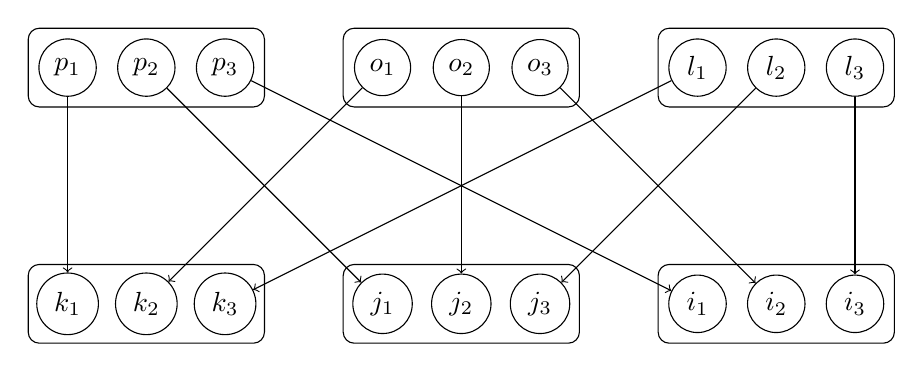
\begin{tikzpicture}
    \draw[rounded corners] (-4.5, 0) rectangle (-1.5, 1) {};
    \node[draw=black, shape=circle, minimum size=0.5cm] (p1) at (-4.0,0.5) {$p_1$};
    \node[draw=black, shape=circle, minimum size=0.5cm] (p2) at (-3.0,0.5) {$p_2$};
    \node[draw=black, shape=circle, minimum size=0.5cm] (p3) at (-2.0,0.5) {$p_3$};

    \draw[rounded corners] (-0.5, 0) rectangle (2.5, 1) {};
    \node[draw=black, shape=circle, minimum size=0.5cm] (o1) at (0.0,0.5) {$o_1$};
    \node[draw=black, shape=circle, minimum size=0.5cm] (o2) at (1.0,0.5) {$o_2$};
    \node[draw=black, shape=circle, minimum size=0.5cm] (o3) at (2.0,0.5) {$o_3$};

    \draw[rounded corners] (3.5, 0) rectangle (6.5, 1) {};
    \node[draw=black, shape=circle, minimum size=0.5cm] (l1) at (4.0, 0.5) {$l_1$};
    \node[draw=black, shape=circle, minimum size=0.5cm] (l2) at (5.0, 0.5) {$l_2$};
    \node[draw=black, shape=circle, minimum size=0.5cm] (l3) at (6.0, 0.5) {$l_3$};

    \draw[rounded corners] (-4.5, -3) rectangle (-1.5, -2) {};
    \node[draw=black, shape=circle, minimum size=0.5cm] (k1) at (-4.0, -2.5) {$k_1$};
    \node[draw=black, shape=circle, minimum size=0.5cm] (k2) at (-3.0, -2.5) {$k_2$};
    \node[draw=black, shape=circle, minimum size=0.5cm] (k3) at (-2.0, -2.5) {$k_3$};

    \draw[rounded corners] (-0.5, -3) rectangle (2.5, -2) {};
    \node[draw=black, shape=circle, minimum size=0.5cm] (j1) at (0.0, -2.5) {$j_1$};
    \node[draw=black, shape=circle, minimum size=0.5cm] (j2) at (1.0, -2.5) {$j_2$};
    \node[draw=black, shape=circle, minimum size=0.5cm] (j3) at (2.0, -2.5) {$j_3$};

    \draw[rounded corners] (3.5, -3) rectangle (6.5, -2) {};
    \node[draw=black, shape=circle, minimum size=0.5cm] (i1) at (4.0, -2.5) {$i_1$};
    \node[draw=black, shape=circle, minimum size=0.5cm] (i2) at (5.0, -2.5) {$i_2$};
    \node[draw=black, shape=circle, minimum size=0.5cm] (i3) at (6.0, -2.5) {$i_3$};

    \draw [->] (p1) -- (k1);
    \draw [->] (p2) -- (j1);
    \draw [->] (p3) -- (i1);
    \draw [->] (o1) -- (k2);
    \draw [->] (o2) -- (j2);
    \draw [->] (o3) -- (i2);
    \draw [->] (l1) -- (k3);
    \draw [->] (l2) -- (j3);
    \draw [->] (l3) -- (i3);

  \end{tikzpicture}
\end{figure}

\subsection{Wyznaczanie liczby $K_{a,b,c,d,e,f}$}
Zakładamy że $m \geq 3$, ponieważ stopień wyjściowy nie może być większy niż 1 a maksymalna liczba wyjściowych krawędzi ze 'zgrupowanego' wierzchołka to 3.

\subsubsection{$H_1$, podział na podzbiory: $\{ a,b,c \}, \{ d,e,f \}$}
Początki krawędzi wychodzących z $p_x, o_x, l_x$ można wybrać na $[m(m-1)(m-2)]^3$ sposobów.
Końce krawędzi prowadzących do jednego z $k_x, j_x, i_x$ można wybrać na:
\begin{itemize}
  \item $m$ sposobów, wtedy jeden stopień wejściowy wynosi 3.
  \item $3m(m-1)$ sposobów, wtedy jeden stopień jest 2 a drugi 1.
  \item $m(m-1)(m-2)$ sposobów, wtedy każdy stopien wynosi 1.
\end{itemize}

\subsubsection{$H_2$, podział na podzbiory: $\{ a,b,d \}, \{ c,e,f \}$}
Początki krawędzi wychodzących z $p_x, o_x, l_x, k_x$ można wybrać na $[m(m-1)(m-2)]^2mm(m-1)$ sposobów.
Końce krawędzi prowadzących do $l_x$ można wybrać na:
\begin{itemize}
  \item $m$ sposobów, wtedy jeden stopień wejściowy wynosi 2.
  \item $m(m-1)$ sposobów, wtedy są dwa stopnie równe 1.
\end{itemize}
Końce krawędzi prowadzących do $k_x$ można wybrać na $m$ sposobów.
Końce krawędzi prowadzących do jednego z $j_x, i_x$ można wybrać na:
\begin{itemize}
  \item $m$ sposobów, wtedy jeden stopień wejściowy wynosi 3.
  \item $3m(m-1)$ sposobów, wtedy jeden stopień jest 2 a drugi 1.
  \item $m(m-1)(m-2)$ sposobów, wtedy każdy stopien wynosi 1.
\end{itemize}

\subsubsection{$H_3$, podział na podzbiory: $\{ a,b,e \}, \{ c,d,f \}$}
Początki krawędzi wychodzących z $p_x,o_x,l_x,k_x$ można wybrać na $m(m-1)(m-2)[m(m-1)]^3$ sposobów. Końce krawędzi prowadzących do jednego z $o_x, l_x, k_x$ można wybrać na $m$ sposobów. Końce prowadzące do $j_x,i_x$ można wybrać na:
\begin{itemize}
  \item $m$ sposobów, wtedy jeden stopień wejściowy wynosi 3.
  \item $3m(m-1)$ sposobów, wtedy jeden stopień jest 2 a drugi 1.
  \item $m(m-1)(m-2)$ sposobów, wtedy każdy stopien wynosi 1.
\end{itemize}

\subsubsection{$H_4$, podział na podzbiory: $\{ a,b,f \}, \{ c,d,e \}$}
Początki krawędzi wychodzących z $p_x,o_x,l_x,k_x$ można wybrać na $m(m-1)(m-2)[m(m-1)]^3$ sposobów. Końce krawędzi prowadzących do jednego z $o_x, l_x, k_x$ można wybrać na $m$ sposobów. Końce prowadzące do $j_x,i_x$ można wybrać na:
\begin{itemize}
  \item $m$ sposobów, wtedy jeden stopień wejściowy wynosi 3.
  \item $3m(m-1)$ sposobów, wtedy jeden stopień jest 2 a drugi 1.
  \item $m(m-1)(m-2)$ sposobów, wtedy każdy stopien wynosi 1.
\end{itemize}

\subsubsection{$H_5$, podział na podzbiory: $\{ a,c,d, \}, \{ b,e,f \}$}
Początki krawędzi wychodzących z $p_x,o_x,l_x,k_x,j_x$ można wybrać na $[m(m-1)(m-2)]^2m^3$ sposoby. Końce krawędzi prowadzących do jednego z $l_x,k_x,j_x$ można wybrać na:
\begin{itemize}
  \item $m$ sposobów, wtedy jeden stopień jest równy 2.
  \item $m(m-1)$ sposobów, wtedy są dwa stopnie równe 1.
\end{itemize}
Końce krawędzi prowadzących do $i_x$ można wybrać na:
\begin{itemize}
  \item $m$ sposobów, wtedy jeden stopień wejściowy wynosi 3.
  \item $3m(m-1)$ sposobów, wtedy jeden stopień jest 2 a drugi 1.
  \item $m(m-1)(m-2)$ sposobów, wtedy każdy stopien wynosi 1.
\end{itemize}

\subsubsection{$H_6$, podział na podzbiory: $\{ a,c,e \}, \{ b,d,f \}$}
Początki krawędzi wychodzących z $p_x, o_x, l_x, k_x, j_x$ można wybrać na $m(m-1)(m-2)[m(m-1)]^2m^2$ sposoby. Końce krawędzi prowadzących do jednego z $o_x, l_x$ można wybrać na $m$ sposobów. Końce krawędzi prowadzących do jednego z $k_x,j_x$ można wybrać na:
\begin{itemize}
  \item $m$ sposobów, wtedy jeden stopień jest równy 2.
  \item $m(m-1)$ sposobów, wtedy są dwa stopnie równe 1.
\end{itemize}
Końce krawędzi prowadzących do $i_x$ można wybrać na:
\begin{itemize}
  \item $m$ sposobów, wtedy jeden stopień wejściowy wynosi 3.
  \item $3m(m-1)$ sposobów, wtedy jeden stopień jest 2 a drugi 1.
  \item $m(m-1)(m-2)$ sposobów, wtedy każdy stopien wynosi 1.
\end{itemize}

\subsubsection{$H_7$, podział na podzbiory: $\{ a,c,f \}, \{ b,d,e \}$}
Początki krawędzi wychodzących z $p_x, o_x, l_x, k_x, j_x$ można wybrać na $m(m-1)(m-2)[m(m-1)]^2m^2$ sposoby. Końce krawędzi prowadzących do jednego z $o_x, l_x$ można wybrać na $m$ sposobów. Końce krawędzi prowadzących do jednego z $k_x,j_x$ można wybrać na:
\begin{itemize}
  \item $m$ sposobów, wtedy jeden stopień jest równy 2.
  \item $m(m-1)$ sposobów, wtedy są dwa stopnie równe 1.
\end{itemize}
Końce krawędzi prowadzących do $i_x$ można wybrać na:
\begin{itemize}
  \item $m$ sposobów, wtedy jeden stopień wejściowy wynosi 3.
  \item $3m(m-1)$ sposobów, wtedy jeden stopień jest 2 a drugi 1.
  \item $m(m-1)(m-2)$ sposobów, wtedy każdy stopien wynosi 1.
\end{itemize}

\subsubsection{$H_8$, podział na podzbiory: $\{ a,d,e \}, \{ b,c,f \}$}
Początki krawędzi wychodzących z $p_x, o_x, l_x, k_x, j_x$ można wybrać na $m(m-1)(m-2)[m(m-1)]^2m^2$ sposobów. Końce krawędzi prowadzących do jednego z $o_x, l_x$ można wybrać na $m$ sposobów. Końce krawędzi prowadzących do jednego z $k_x,j_x$ można wybrać na:
\begin{itemize}
  \item $m$ sposobów, wtedy jeden stopień jest równy 2.
  \item $m(m-1)$ sposobów, wtedy są dwa stopnie równe 1.
\end{itemize}
Końce krawędzi prowadzących do $i_x$ można wybrać na:
\begin{itemize}
  \item $m$ sposobów, wtedy jeden stopień wejściowy wynosi 3.
  \item $3m(m-1)$ sposobów, wtedy jeden stopień jest 2 a drugi 1.
  \item $m(m-1)(m-2)$ sposobów, wtedy każdy stopien wynosi 1.
\end{itemize}

\subsubsection{$H_9$, podział na podzbiory: $\{ a,d,f \}, \{ b,c,e \}$}
Początki krawędzi wychodzących z $p_x, o_x, l_x, k_x, j_x$ można wybrać na $m(m-1)(m-2)[m(m-1)]^2m^2$ sposobów. Końce krawędzi prowadzących do jednego z $o_x, l_x$ można wybrać na $m$ sposobów. Końce krawędzi prowadzących do jednego z $k_x,j_x$ można wybrać na:
\begin{itemize}
  \item $m$ sposobów, wtedy jeden stopień jest równy 2.
  \item $m(m-1)$ sposobów, wtedy są dwa stopnie równe 1.
\end{itemize}
Końce krawędzi prowadzących do $i_x$ można wybrać na:
\begin{itemize}
  \item $m$ sposobów, wtedy jeden stopień wejściowy wynosi 3.
  \item $3m(m-1)$ sposobów, wtedy jeden stopień jest 2 a drugi 1.
  \item $m(m-1)(m-2)$ sposobów, wtedy każdy stopien wynosi 1.
\end{itemize}

\subsubsection{$H_{10}$, podział na podzbiory: $\{ a,e,f \}, \{ b,c,d \}$}
Początki krawędzi wychodzących z $p_x, o_x, l_x, k_x, j_x$ można wybrać na $[m(m-1)(m-2)]^2m^3$ sposoby. Końce krawędzi prowadzących do jednego z $l_x, k_x, j_x$ można wybrać na:
\begin{itemize}
  \item $m$ sposobów, wtedy jeden stopień jest równy 2.
  \item $m(m-1)$ sposobów, wtedy są dwa stopnie równe 1.
\end{itemize}
Końce krawędzi prowadzących do $i_x$ można wybrać na:
\begin{itemize}
  \item $m$ sposobów, wtedy jeden stopień wejściowy wynosi 3.
  \item $3m(m-1)$ sposobów, wtedy jeden stopień jest 2 a drugi 1.
  \item $m(m-1)(m-2)$ sposobów, wtedy każdy stopien wynosi 1.
\end{itemize}
Przypadki $H_3, H_4$ oraz $H_6, H_7, H_8, H_9$ są tożsame.

\subsection{Wyznaczanie prawdopodobieństwa $p_{K_{a,b,c,d,e,f}}$}
Ponieważ liczba krawędzi $H$ jest stała to liczba $C_H$ jest ograniczona z góry przez stałą.
Gdy $n$ jest wystarczająco duże to ilorazy $\frac{C_H(i)^2}{i}$ będą bliskie zeru zatem ostatni z 3 czynników iloczynu można zaniedbać:
\begin{dmath}
  p_{K_{a,b,c,d,e,f}^*} = (\prod_{v \in V^{-}(H)} d_{H}^{in}(v)!) \frac{1}{2^{9}} \frac{1}{\sqrt{m^{18} a^3 b^3 c^3 d^3 e^3 f^3}} 
  = (\prod_{v \in V^{-}(H)} d_{H}^{in}(v)!) \frac{1}{2^{9}} \frac{1}{m^{9} a^{\frac{3}{2}} b^{\frac{3}{2}} c^{\frac{3}{2}} d^{\frac{3}{2}} e^{\frac{3}{2}} f^{\frac{3}{2}}}
\end{dmath} 

\subsection{Wyznaczanie oczekiwanej liczby $K_{3,3}$}

\begin{dmath}
  \mathbb{E}[K_{3,3}] = \sum_{K_{3,3}^* \in \mathbb{K}_{3,3}} \sum_{1 \leq a < b < c < d < e < f \leq n} \#K_{a,b,c,d,e,f}^* \cdot p_{K_{a,b,c,d,e,f}^*}
  = \sum_{K_{3,3}^* \in \mathbb{K}_{3,3}} (\prod_{v \in V^{-}(H)} d_{H}^{in}(v)!) \cdot \frac{1}{2^{9} m^{9}} \cdot \#K_{a,b,c,d,e,f}^* \sum_{1 \leq a < b < c < d < e < f \leq n} \frac{1}{a^{\frac{3}{2}} b^{\frac{3}{2}} c^{\frac{3}{2}} d^{\frac{3}{2}} e^{\frac{3}{2}} f^{\frac{3}{2}}}
  = \sum_{K_{3,3}^* \in \mathbb{K}_{3,3}} [(\prod_{v \in V^{-}(H)} d_{H}^{in}(v)!) \cdot \frac{1}{2^{9} m^{9}} \cdot \#K_{a,b,c,d,e,f}^*] \cdot (\frac{1}{6!})^{\frac{3}{2}} \cdot (H^{\frac{3}{2}}_n)^6
\end{dmath}
gdzie $H^{\frac{3}{2}}_n$ to n-ta liczba harmoniczna rodzaju $\frac{3}{2}$.
\newline \newline
Ostatecznie oczekiwana liczba $K_{3,3}$ w grafie $G_m^n$ wynosi:
\begin{dmath}
  \mathbb{E}[K_{3,3}] = \frac{(m^2-1)^2(5m^8-35m^6+74m^4-64m^2+32)}{2211840 \sqrt{5} m^3} (H^{\frac{3}{2}}_n)^6
\end{dmath}

\newpage

\subsection{Eksperyment}
Dla stałej $\eta \approx \frac{1}{1.6}$ tak prezentuje się porównanie teorii $\eta \cdot \mathbb{E}[K_{3,3}]$ i eksperymentu:

\begin{figure}[h!]
  \centering
  \includegraphics[width=13cm]{../k33.png}
  \caption{Porównanie teorii i eksperymentu dla $K_{3,3}$ - 100 prób}
\end{figure}

\newpage

\section{Oczekiwana liczba podgrafów będących podpodziałami pewnego grafu $F$}
Podpodziały powstają poprzez dodawanie wierzchołków stopnia 2 na istniejących krawędziach.
\newline
Niech $v_1, \ldots v_k$, będą wierzchołkami w $G_m^n$ tworzącymi potencjalny podpodział $F$.
Bierzemy graf $G = G_1^{n \cdot m}$ oraz graf  $H$ będący pewnym podpodziałem $F$.
\subsection{Wyznaczanie liczby podpodziałów $F$ zbudowanych na $k$ wierzchołkach}
Spośród wierzchołków $v_1, \ldots v_k$ wybieramy $|V(F)|$ wierzchołków, które stworzą graf $F$. Robimy to na $\binom{k}{|V(F)|}$ sposobów.
Następnie pozostałe wierzchołki rozdzielamy na $|E(F)|$ krawędzi. Rozdzieleń tych wierzchołków na $|E(F)|$ grup jest $\binom{k'+|E(F)|-1}{|E(F)|-1}$, gdzie $k' = k-|V(F)|$. Każdy podział daje nam rozbicie $k'=k_1 + k_2 + \ldots + k_{|E(F)|}$, gdzie $k_i$ to liczba wierzchołków przyporządkowana do $i$-tej krawędzi.
Następnie podział na dane rozbicie możemy zrealizować na $\frac{k'!}{k_1! \cdot k_2! \ldots k_{|E(F)|}!}$ sposobów.
Wierzchołki w każdej krawędzi można ustawić na $k_i!$ sposobów. Zatem różnych podziałów jest:
\begin{dmath}
  \binom{k'+|E(F)|-1}{|E(F)|-1} \cdot \frac{k'!}{k_1! \cdot k_2! \ldots k_{|E(F)|}!} \cdot k_1! \cdot k_2! \ldots k_{|E(F)|}! = \binom{k'+|E(F)|-1}{|E(F)|-1} \cdot k'!
\end{dmath}
Więc różnych podpodziałów $F$ jest:
\begin{dmath}
 \#F_k = \binom{k}{|V(F)|} \cdot \#F \cdot \binom{k-|V(F)|+|E(F)|-1}{|E(F)|-1} \cdot (k-|V(F)|)!
\end{dmath}

\subsection{Wyznaczanie prawdopodobieństwa $p_{F_k}$}
Dodanie ciągu wierzchołków stopnia 2 na krawędziach grafu $F$ w rozważanym modelu dodaje nam 'zgrupowane' wierzchołki, które mają:
\begin{enumerate}
  \item jeden stopień wejściowy i jeden stopień wyjściowy, dla wierzchołków których jeden sąsiad ma wyższy numer a drugi niższy.
  \item dwa stopnie wyjściowe, dla wierzchołków których obaj sąsiedzi mają niższe numery.
  \item dwa stopnie wejściowe, dla wierzchołków których obaj sąsiedzi mają wyższe numery.
\end{enumerate}
W 1. przypadku mamy $m \cdot m$ możliwości, w 2. $m \cdot (m-1)$ a w 3. $m \cdot m$. W pierwszym i drugim przypadku stopnie wejściowe nie przekraczają 1, w trzecim przypadku nie przekraczają 1. W 3. przypadku jest $m$ sytuacji, gdzie stopień wejściowy wynosi 2 a w pozostałych $m(m-1)$ 2 stopnie wynoszą 1.

\subsubsection{Oczekiwana liczba przypadków 1., 2., 3.}
Dla każdego wierzchołka $i$ niebędącego w $V(F)$ definujemy zmienną losową $X^w_i$ taką, że:
\begin{itemize}
  \item 1, gdy $i$ spełnia warunek z punktu $w$
  \item 0, w przeciwnym przypadku
\end{itemize}
Oczekiwana liczba wierzchołków spełniających warunek $w$ wynosi $\mathbb{E}[X^w_i] = \frac{1}{3}$, ponieważ dany wierzchołek $i$ i jego sąsiedztwo reprezentują 3 różne liczby. 
Mogą one być w relacji ze sobą na 6 sposobów, z których 2 spełniają warunek 1., 2. lub 3.
Wówczas oczekiwana liczba wierzchołków spełniających warunek 3. wynosi(zakładamy niezależność zmiennych losowych):
\begin{dmath}
  \mathbb{E}[\sum_{i \notin V(F)} X^w_i] = \sum_{i \notin V(F)} \mathbb{E}[X^w_i] = \frac{k-|V(F)|}{3}
\end{dmath}
Dodanie wierzchołków stopnia 2 wpływa na stopnie grafu $F$, ale że $F$ jest mały to wpływ jest znikomy.
\newline \newline
Należy także określić liczbę $C_{F_k}$ - liczbę krawędzi $(i,j)$ takich, że $i \leq t \leq j$.
Dla każdego wierzchołka $t$ z $V(F)$ mamy maksymalnie $t-1$ wierzchołków o numerach mniejszych od $t$ oraz $k-t$ wierzchołków o numerach większych od $t$
co przekłada się na prawdopodobieństwo $\frac{t-1}{k} \cdot \frac{k-t}{k-1}$ trafienia na parę zliczaną przez $C_{F_k}$.
Maksymalnie takich par może być $k-1$ zatem oczekiwana liczba $C_{F_k}$ wynosi:
\begin{dmath}
  \mathbb{E}[C_{F_k}] = (k-1) \cdot \frac{t-1}{k} \cdot \frac{k-t}{k-1} = \frac{(t-1)(k-t)}{k}
\end{dmath}
Co przekłada się na:
\begin{dmath}
  O(\exp(\sum_{t \in V(F_k)}\frac{C_{F_k}(t)^2}{t})) = O(\exp(\sum_{t=1}^{k} \frac{(t-1)^2(k-t)^2}{k^2})) = O(\exp(k^2)),
\end{dmath}
Ale formułę z notacją $O(\cdot)$ można zamienić na dokładną formułę:
\begin{dmath}
  p_H = \prod_{v \in V^{-}(H)} d_{H}^{in}(v)! \prod_{v \in V^{+}(H)} \frac{1}{2v - 1} \prod_{v \notin V^{+}(H)} (1 + \frac{C_{H}(v)}{2v-1})
\end{dmath}
Wtedy ostatni czynnik można zapisać jako 
\begin{dmath}
  \prod_{t \notin V^{+}(H)} (1 + \frac{\frac{(t-1)(k-t)}{k}}{2t-1}) =
  \prod_{t \notin V^{+}(H)} (1 + \frac{k-t}{2k}) =
  \prod_{t \notin V^{+}(H)} (\frac{3}{2} - \frac{t}{2k}) \leq (\frac{3}{2})^{\frac{k}{2}}
\end{dmath}
Mając konkretne ustawienie $k$ wierzchołków wyznaczamy $p_{F_k}$ przemnożone dla różnych rozłożeń stopni.
Na podstawie opisanych wyżej 3. przypadków mamy 2 możliwości rozdziału stopni.
\newline
\textbf{Wszystkie stopnie są nie większe niż 1:}
\newline
Jest ich $(m^2)^{\frac{k'}{3}} \cdot (m(m-1))^{\frac{k'}{3}} \cdot (m(m-1))^{\frac{k'}{3}} = (m^4(m-1)^2)^{\frac{k'}{3}} \approx (m^2)^{k'}$
\begin{dmath}
  p_{F_k^1} = \frac{1}{2^{k'}} \cdot \frac{1}{v_{i_1} \cdot \ldots \cdot v_{i_{k'}} \cdot m^{k'}} \cdot (\frac{3}{2})^{\frac{k'}{3}}
\end{dmath}
\textbf{Występują stopnie 2 - opsane w przypadku 3.:}
\newline
Jest ich $(m^2)^{\frac{k'}{3}} \cdot (m(m-1))^{\frac{k'}{3}} \cdot m^{\frac{k'}{3}} = (m^4(m-1))^{\frac{k'}{3}} \approx (m^{\frac{5}{3}})^{k'}$
\begin{dmath}
  p_{F_k^2} = 2^{\frac{k'}{3}} \cdot \frac{1}{2^{k'}} \cdot \frac{1}{v_{i_1} \cdot \ldots \cdot v_{i_{k'}} \cdot m^{k'}} \cdot (\frac{3}{2})^{\frac{k'}{3}}
\end{dmath}
Co możemy połączyć w jedno wyrażenie określające oczekiwane $F_k$ dla konkretnego ustawienia wierzchołków $v_1, \ldots v_k$ - $\mathbb{E}[F_k^\#]$:
\begin{dmath}
  \mathbb{E}[F_k^\#] = (m^2)^{k'} \cdot \frac{1}{2^{k'}} \cdot \frac{1}{v_{i_1} \cdot \ldots \cdot v_{i_{k'}} \cdot m^{k'}} \cdot (\frac{3}{2})^{\frac{k'}{3}} +
  (m^{\frac{5}{3}})^{k'} \cdot 2^{\frac{k'}{3}} \cdot \frac{1}{2^{k'}} \cdot \frac{1}{v_{i_1} \cdot \ldots \cdot v_{i_{k'}} \cdot m^{k'}} \cdot (\frac{3}{2})^{\frac{k'}{3}} = 
  (m^{k'} + (2m^2)^{\frac{k'}{3}}) \cdot \frac{1}{2^{k'}} \cdot (\frac{3}{2})^{\frac{k'}{3}} \cdot \frac{1}{v_{i_1} \cdot \ldots \cdot v_{i_{k'}}}
\end{dmath}
Gdy $v_{i_1} < \ldots < v_{i_{k'}}$ wybierzemy z $n$ wierzchołków to otrzymamy:
\begin{dmath}
  \mathbb{E}[F_k^*] = \sum_{1 \leq v_1 < \ldots < v_k \leq n} \mathbb{E}[F_k^\#] = 
  (m^{k'} + (2m^2)^{\frac{k'}{3}}) \cdot \frac{1}{2^{k'}} \cdot (\frac{3}{2})^{\frac{k'}{3}} \cdot \frac{1}{k!} \cdot H_n^{k'} =
  (m^{k'} + (2m^2)^{\frac{k'}{3}}) \cdot \frac{1}{2^{k'}} \cdot (\frac{3}{2})^{\frac{k'}{3}} \cdot \frac{1}{k!} \cdot log_2(n)^{k'}
\end{dmath}

\subsection{Wyznaczanie oczekiwanej liczby $F_k$}
Wystarczy już tylko przemnożyć $\mathbb{E}[F_k^*]$ przez $\#F_k$ i zsumować po $k=1, \ldots, n$:
\begin{dmath}
  \mathbb{E}[F] = \sum_{k=1}^n \#F_k \cdot \mathbb{E}[F_k^*]
\end{dmath}

\subsection{Wizualizacja $\mathbb{E}[F_k^*]$}
Zmiana wartości dla różnych $k \in \{1, \ldots, 25\}$ dla $m=2$ i $n=1000$:
\begin{figure}[h!]
  \centering
  \includegraphics[width=13cm]{../fk.png}
\end{figure}

\section{Obserwacje}
\begin{itemize}
  \item Model BA nie jest skłonny do planarności
  \item Dla $m=1$ w grafie nie powstają cykle, więc nie ma powodów do nieplanarności
  \item Dla $m>1$ grafy szybko stają się nieplanarne
  \item Powodem nieplanarności częściej są podpodziały $K_{3,3}$ niż $K_5$
  \item Podpodziałami najczęściej występującymi są te zbudowane na $(\log_2(n) + 5) \cdot O(m^x)$ wierzchołkach - obserwacja ostatnich wizualizacji. Zatem podpodziałów należy szukać w podgrafach rozmiarów $O(\log_2(n))$.
\end{itemize}

\end{document}
